% Original source: Zhou, physical PDF pp. 168--172 (printed pp. 152--156).
% Figures 6.3 and 6.4 are recreated as native TikZ diagrams.

% ZHOU-SOURCE-PAGE: 168 PRINTED: 152

unit of option) in the money market. If there is a sudden increase in $S$, $d_1$ increases and
$\Delta$ increases as well. That means we need to short more stock and lend more cash
($Ke^{-r\tau}N(d_2)$ also increases).

The delta hedge only replicates the value and the slope of the option. To hedge the
curvature of the option, we will need to hedge gamma as well.

\end{solution}

\begin{problem}{D. Can you estimate the value of an at-the-money call on a non-dividend paying stock?
Assume the interest rate is low and the call has short maturity.}
\end{problem}

\begin{solution}
When $S=K$, we have $c=S\left(N(d_1)-e^{-r\tau}N(d_2)\right)$. In a low-interest
environment, $r\approx0$ and $e^{-r\tau}\approx1$, so
$c\approx S\left(N(d_1)-N(d_2)\right)$.

We also have

\[
N(d_1)-N(d_2)=\int_{d_2}^{d_1}\frac{1}{\sqrt{2\pi}}e^{-x^2/2}\,\dd x,
\]

where

\[
d_2=\left(\frac{r}{\sigma}-\frac{\sigma}{2}\right)\sqrt{\tau}
\qquad\text{and}\qquad
d_1=\left(\frac{r}{\sigma}+\frac{\sigma}{2}\right)\sqrt{\tau}.
\]

For a small $r$, a typical $\sigma$ for stocks ($<40\%$ per year) and a short maturity
($<3$ months), both $d_2$ and $d_1$ are close to 0. For example, if $r=0.03$,
$\sigma=0.3$, and $\tau=1/6$ year, then
$d_2=-0.02$ and $e^{-d_2^2/2}=0.98$.

\[
\begin{aligned}
\therefore\quad N(d_1)-N(d_2)&\approx\frac{1}{\sqrt{2\pi}}(d_1-d_2)\\
&=\frac{\sigma\sqrt{\tau}}{\sqrt{2\pi}}\\
&\approx0.4\sigma\sqrt{T-t}\Rightarrow c\approx0.4\sigma S\sqrt{\tau}.
\end{aligned}
\]

\noindent\emph{In practice, this approximation is used by some volatility traders to estimate
the implied volatility of an at-the-money option.}

(The approximation $e^{-x^2/2}\approx1$ causes a small overestimation since
$e^{-x^2/2}<1$, but the approximation $-e^{-r\tau}K\approx-K$ causes a small
underestimation. To some extent, the two opposite effects cancel out and the overall
approximation is fairly accurate.)

\end{solution}

\subsubsection*{Gamma}

For a European call/put with dividend yield $y$:

\[
\Gamma=\frac{N'(d_1)e^{-y\tau}}{S_0\sigma\sqrt{\tau}}
\]

% ZHOU-SOURCE-PAGE: 169 PRINTED: 153

\begin{problem}{What happens to the gamma of an at-the-money European option when it approaches
its maturity?}
\end{problem}

\begin{solution}
From the put-call parity, it is obvious that a call and a put with identical
characteristics have the same gamma (since $\Gamma=0$ for both the cash position and the
underlying stock). Taking the partial derivative of the $\Delta$ of a call option with
respect to $S$, we have

\[
\Gamma=\frac{N'(d_1)e^{-y\tau}}{S\sigma\sqrt{\tau}},
\qquad\text{where}\qquad
N'(d_1)=\frac{1}{\sqrt{2\pi}}e^{-d_1^2/2}.
\]

\noindent\emph{So for plain vanilla call and put options, gamma is always positive.}

Figure 6.3 shows that gamma is high when options are at the money, which is the stock
price region that $\Delta$ changes rapidly with $S$. If $S\ll K$ or $S\gg K$ (deep in the
money or out of the money), gamma approaches 0 since $\Delta$ stays constant at 1 or 0.
The gamma of options with shorter maturities approaches 0 much faster than options with
longer maturities as $S$ moves away from $K$. So for deep in-the-money or deep
out-of-the-money options, longer maturity means higher gamma. In contrast, if the stock
prices are close to the strike price (at the money) as the maturity nears, the slope of delta
for an at-the-money call becomes steeper and steeper. So for options close to the strike
price, shorter-term options have higher gammas.

As $\tau\to0$, an at-the-money call/put has $\Gamma\to\infty$ ($\Delta$ becomes a step
function). This can be shown from the formula of gamma for a European call/put with no
dividend,

\[
\Gamma=\frac{N'(d_1)}{S\sigma\sqrt{\tau}}.
\]

When $S=K$,

\[
\begin{aligned}
d_1&=\lim_{\tau\to0}\left(\frac{r}{\sigma}+\frac{\sigma}{2}\right)\sqrt{\tau}\\
&\to0\Rightarrow\lim_{\tau\to0}N'(d_1)\to\frac{1}{\sqrt{2\pi}}.
\end{aligned}
\]

The numerator is $1/\sqrt{2\pi}$; yet the denominator has a limit
$\lim_{\tau\to0}S\sigma\sqrt{\tau}\to0$, so $\Gamma\to\infty$. In other words, When
$\tau=T$, delta becomes a step function. This phenomenon makes hedging at-the-money
options difficult when $t\to T$ since delta is extremely sensitive to changes in $S$.

% ZHOU-SOURCE-PAGE: 170 PRINTED: 154

\begin{figure}[ht]
\centering
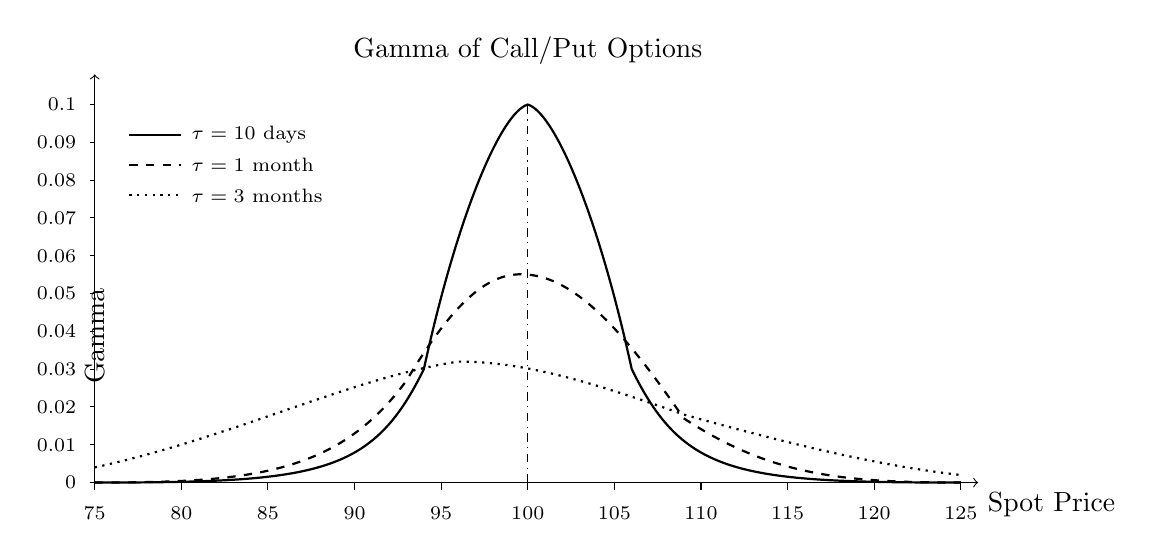
\begin{tikzpicture}[x=0.22cm,y=48cm]
  \draw[->] (75,0) -- (126,0) node[below right] {Spot Price};
  \draw[->] (75,0) -- (75,0.108) node[midway,left,rotate=90] {Gamma};
  \node[above] at (100,0.108) {Gamma of Call/Put Options};
  \foreach \x in {75,80,85,90,95,100,105,110,115,120,125}{
    \draw (\x,0) -- (\x,-0.002);
    \node[below] at (\x,-0.004) {\scriptsize \x};
  }
  \foreach \y/\lab in {0/0,0.01/0.01,0.02/0.02,0.03/0.03,0.04/0.04,0.05/0.05,
    0.06/0.06,0.07/0.07,0.08/0.08,0.09/0.09,0.1/0.1}{
    \draw (74.7,\y) -- (75,\y);
    \node[left] at (74.5,\y) {\scriptsize \lab};
  }
  \draw[dash dot] (100,0) -- (100,0.1);
  \draw[thick] (75,0) .. controls (88,0) and (91,0.002) .. (94,0.03)
    .. controls (96,0.072) and (98.5,0.098) .. (100,0.1)
    .. controls (101.5,0.098) and (104,0.072) .. (106,0.03)
    .. controls (109,0.002) and (112,0) .. (125,0);
  \draw[dashed,thick] (75,0) .. controls (84,0) and (89,0.002) .. (93,0.027)
    .. controls (96,0.05) and (98,0.056) .. (100,0.055)
    .. controls (103,0.054) and (106,0.037) .. (109,0.017)
    .. controls (114,0.002) and (118,0) .. (125,0);
  \draw[dotted,thick] (75,0.004) .. controls (83,0.012) and (90,0.028) .. (96,0.032)
    .. controls (100,0.032) and (104,0.026) .. (109,0.018)
    .. controls (116,0.009) and (121,0.004) .. (125,0.002);
  \draw[thick] (77,0.092) -- (80,0.092) node[right] {\scriptsize $\tau=10$ days};
  \draw[dashed,thick] (77,0.084) -- (80,0.084) node[right] {\scriptsize $\tau=1$ month};
  \draw[dotted,thick] (77,0.076) -- (80,0.076) node[right] {\scriptsize $\tau=3$ months};
\end{tikzpicture}
\caption{Variation of gamma of a European call option with respect to $S$ and
$T$. $K=100$, $r=0.05$, $\sigma=0.25$.}
\label{fig:zhou-figure-6-3}
\end{figure}

\end{solution}

\subsubsection*{Theta}

For a European call option:

\[
\begin{aligned}
\Theta&=-\frac{SN'(d_1)\sigma e^{-y\tau}}{2\sqrt{\tau}}\\
&\quad+ySe^{-y\tau}N(d_1)-rKe^{-r\tau}N(d_2)
\end{aligned}
\]

For a European put option:

\[
\begin{aligned}
\Theta&=-\frac{SN'(d_1)\sigma e^{-y\tau}}{2\sqrt{\tau}}\\
&\quad-ySe^{-y\tau}N(-d_1)+rKe^{-r\tau}N(-d_2)
\end{aligned}
\]

When there is no dividend, the theta for a European call option is simplified to

\[
\Theta=-\frac{SN'(d_1)}{2\sqrt{\tau}}-rKe^{-r\tau}N(d_2),
\]

which is always negative. As shown in Figure 6.4, when $S\ll K$, $N(d_2)\approx0$ and
$N'(d_1)\approx0$. Hence, $\Theta\to0$. When $S\gg K$, $N(d_2)\approx1$ and

% ZHOU-SOURCE-PAGE: 171 PRINTED: 155

$N'(d_1)\approx0$. Hence, $\Theta\to-rKe^{-r\tau}$. When $S\approx K$, $\Theta$ has
large negative value and the smaller the $\tau$, the more negative the $\Theta$.

\begin{figure}[ht]
\centering
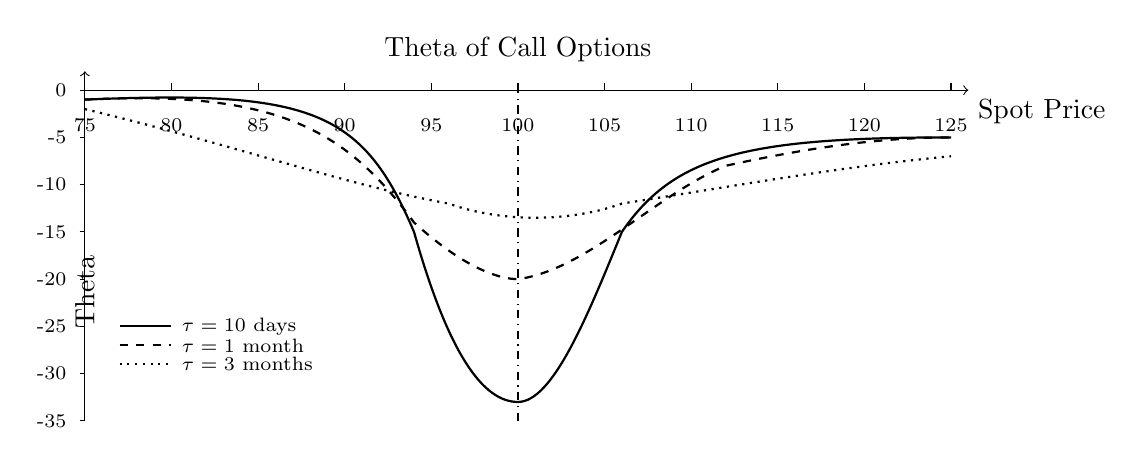
\begin{tikzpicture}[x=0.22cm,y=0.12cm]
  \draw[->] (75,0) -- (126,0) node[below right] {Spot Price};
  \draw[->] (75,-35) -- (75,2) node[midway,left,rotate=90] {Theta};
  \node[above] at (100,2) {Theta of Call Options};
  \foreach \x in {75,80,85,90,95,100,105,110,115,120,125}{
    \draw (\x,0) -- (\x,0.8);
    \node[below] at (\x,-2) {\scriptsize \x};
  }
  \foreach \y in {0,-5,-10,-15,-20,-25,-30,-35}{
    \draw (74.7,\y) -- (75,\y);
    \node[left] at (74.5,\y) {\scriptsize \y};
  }
  \draw[dash dot] (100,-35) -- (100,0);
  \draw[thick] (75,-1) .. controls (88,0) and (91,-2) .. (94,-15)
    .. controls (96,-28) and (98,-33) .. (100,-33)
    .. controls (102,-33) and (104,-24) .. (106,-15)
    .. controls (109,-7) and (113,-5) .. (125,-5);
  \draw[dashed,thick] (75,-1) .. controls (86,0) and (90,-4) .. (94,-14)
    .. controls (97,-19) and (99,-20) .. (100,-20)
    .. controls (104,-19) and (108,-11) .. (112,-8)
    .. controls (117,-6) and (121,-5) .. (125,-5);
  \draw[dotted,thick] (75,-2) .. controls (84,-6) and (90,-10) .. (96,-12)
    .. controls (99,-14) and (103,-14) .. (106,-12)
    .. controls (113,-10) and (119,-8) .. (125,-7);
  \draw[thick] (77,-25) -- (80,-25) node[right] {\scriptsize $\tau=10$ days};
  \draw[dashed,thick] (77,-27) -- (80,-27) node[right] {\scriptsize $\tau=1$ month};
  \draw[dotted,thick] (77,-29) -- (80,-29) node[right] {\scriptsize $\tau=3$ months};
\end{tikzpicture}
\caption{Variation of theta of a European call option with respect to $S$ and
$T$. $K=100$, $\sigma=0.25$, $r=0.05$.}
\label{fig:zhou-figure-6-4}
\end{figure}

\begin{problem}{A. When will a European option have positive theta?}
\end{problem}

\begin{solution}
For American options as well as European calls on non-dividend paying assets, theta is
always negative. But for deep in-the-money European puts, their values may increase as
$t$ approaches $T$ if all other factors remain the same, so they may have positive theta.

A put option on a non-dividend paying asset has

\[
\Theta=-\frac{SN'(d_1)\sigma}{2\sqrt{\tau}}+rKe^{-r\tau}N(-d_2).
\]

If the put option is deep in-the-money ($S\ll K$), then $N'(d_1)\approx0$ and
$N(-d_2)\approx1$. Hence,

% ZHOU-SOURCE-PAGE: 172 PRINTED: 156

$\Theta\approx rKe^{-r\tau}>0$. That's also the reason why it can be optimal to exercise a
deep in-the-money American put before maturity.

For deep in-the-money European call options with high dividend yield, the theta can be
positive as well. If a call option with high dividend yield is deep in-the-money
($S\gg K$), $N(d_1)\approx N(d_2)\approx1$, $N'(d_1)\approx0$, so the component
$ySe^{-y\tau}N(d_1)$ can make $\Theta$ positive.

\end{solution}

\begin{problem}{B. You just entered a long position for a call option on GM and hedged the position
by shorting GM shares to make the portfolio delta neutral. If there is an immediate increase
or decrease in GM's stock price, what will happen to the value of your portfolio? Is it an
arbitrage opportunity? Assume that GM does not pay dividends.}
\end{problem}

\begin{solution}
A position in the underlying asset has zero gamma. So the portfolio is delta-neutral and
long gamma. Therefore, either an immediate increase or decrease in the GM stock price
will increase the portfolio value. The convexity (positive gamma) enhances returns when
there is a large move in the stock price in either direction.

Nevertheless, it is not an arbitrage opportunity. It is a trade-off between gamma and theta
instead. From the Black-Scholes-Merton differential equation, the portfolio $V$ satisfies
the equation

\[
\begin{aligned}
\frac{\partial V}{\partial t}+rS\frac{\partial V}{\partial S}
&+\frac{1}{2}\sigma^2S^2\frac{\partial^2V}{\partial S^2}\\
&=\Theta+rS\Delta+\frac{1}{2}\sigma^2S^2\Gamma=rV.
\end{aligned}
\]

For a delta-neutral portfolio, we have

\[
\Theta+\frac{1}{2}\sigma^2S^2\Gamma=rV.
\]

This indicates that gamma and theta often have opposite signs. For example, when an
at-the-money call approaches maturity, gamma is large and positive, so theta is large and
negative. Our delta neutral portfolio has positive gamma and negative theta. That means if
the price does not move, the passage of time will result in a lower portfolio value unless we
rebalance. So the portfolio does not provide an arbitrage opportunity.

\end{solution}

\subsubsection*{Vega}

For European options:

\[
\begin{aligned}
\nu&=\frac{\partial c}{\partial\sigma}=\frac{\partial p}{\partial\sigma}\\
&=Se^{-y\tau}\sqrt{\tau}\,N'(d_1)
\end{aligned}
\]

At-the-money options are most sensitive to volatility change, so they have higher vegas
than either in-the-money or out-of-the-money options. The vegas of all options decrease as
time to expiration becomes shorter ($\sqrt{\tau}\to0$) since a long-term option is more
sensitive to change in volatility.

\begin{problem}{A. Explain implied volatility and volatility}
